\documentclass{article}
\usepackage[utf8]{inputenc}
\usepackage[export]{adjustbox}
\usepackage{geometry}
\usepackage{amsmath, amssymb}
\usepackage{listings}
\usepackage{graphicx}
\usepackage{float}
\usepackage{booktabs}
\usepackage{hyperref}
\usepackage{titlesec}
\usepackage{listings}
\usepackage{makecell}
\usepackage{array}
\usepackage{xcolor}
\usepackage{minted}

% Define absolute value command
\newcommand{\abs}[1]{\left|#1\right|}

% Define partial derivative command
\newcommand{\pderiv}[2]{\frac{\partial #1}{\partial #2}}

% Define norm command
\newcommand{\norm}[1]{\left\lVert#1\right\rVert}

% Define background color for the code block
\definecolor{backgroundColor}{rgb}{0.95, 0.95, 0.95}

% minted settings
\setminted{
    bgcolor=backgroundColor,
    linenos,
    frame=lines,
    framesep=5pt,
    fontsize=\small
}

% Graphic Path settings
\graphicspath{{/Volumes/Bi/HUST/SOICT-HUST ICT Program/Object Oriented Programming/Project/image}}

% Geometry settings
\geometry{a4paper, margin=1in}

% Section formatting
\titleformat{\section}{\bfseries\large}{\thesection}{1em}{}
\titleformat{\subsection}{\bfseries\normalsize}{\thesubsection}{1em}{}

% Hyperlink settings
\hypersetup{
    colorlinks=true,
    linkcolor=blue,
    urlcolor=blue,
    pdftitle={Chap5 Notes},
    pdfauthor={},
    pdfcreator={LaTeX}
}

% Prevent automatic page breaks after minted blocks
\setlength{\parskip}{0pt}  % No paragraph skip after the block
\setlength{\parindent}{0pt} % No paragraph indent

\begin{document}

% --- TITLE PAGE ---
\begin{titlepage}
    \centering
    \vspace{0.5cm} % Adjust as needed
    {\LARGE\bfseries Hanoi University of Science and Technology}\\[0.5em]
    {\Large School of Information and Communication Technology}

    \vspace{0.2cm}
    \rule{\textwidth}{0.4pt}
    \vspace{2.5cm}

    % Logos
    \centering
    
\includegraphics[width=0.8\textwidth]{soict.png} % Replace with actual SOICT logo


    \vspace{2cm} % Adjust spacing

    {\huge\bfseries Project Report}\\[0.5em]
    {\LARGE\bfseries Object-Oriented Programming}\\[1em]

    {\LARGE\bfseries Quick Lap}\\[1em]

    {\Large Topic: Laptop Recommendation System}\\[0.5em]
    {\large Integrated Information Retrieval and Large Language Model}

    \vfill % Pushes content downwards

    \begin{tabular}{@{}ll}
        \textbf{Group:}      & 7 \\
        \addlinespace[0.5em]
        \textbf{Members:}    & Nguyen Tuan Duong \hspace{2em} 20235924 \\
                             & Nguyen Duc Anh \hspace{2.7em} 20235890 \\ % Manual spacing for alignment
                             & Hoang Quoc Cuong \hspace{1.9em} 20235903 \\
                             & Nguyen Minh Duc \hspace{2em} 20235915 \\
                             & Pham Minh Duc \hspace{2.7em} 20235918 \\
        \addlinespace[0.5em]
        \textbf{Supervisor:} & TS. Trinh Tuan Dat
    \end{tabular}
    \vfill
    \vspace{1cm} 
    {\large Hanoi, 5/2025}
\end{titlepage}

\pagenumbering{arabic} % Start page numbering for content
\setcounter{page}{2} % To match the PDF's numbering (ToC is page 2)

% --- CONTRIBUTION ---
\section*{Contribution}
\begin{table}[H]
\renewcommand{\arraystretch}{2}
\noindent 
\raggedright
\resizebox{\textwidth}{!}
{
\begin{tabular}{|c|c|c|}
    \hline
    Nguyen Tuan Duong - 20235924 & Implement RAG; Slide Maker & 20\% \\
    \hline
    Nguyen Duc Anh - 20235890 & Implement Laptop, Product class; Write Report; Design Use-Case and UML Diagram & 20\% \\
    \hline
    Nguyen Minh Duc - 20235915 & Implement UI controller, FXML & 20\% \\
    \hline
    Pham Minh Duc - 20235918 & Implement DataCollector & 20\% \\
    \hline
    Hoang Quoc Cuong - 20235903 & Implement Database, Design Searching Algorithms & 20\% \\
    \hline
\end{tabular}
}
\end{table}

% --- TIMELINE ---
\section*{TimeLine}
\begin{itemize}
    \item \textbf{March (Approx.): Phase 1 - Ideation, Research \& Planning}
    \begin{itemize}
        \item Proposal development and finalization of project ideas.
        \item In-depth research into implementation methodologies, covering:
        \begin{itemize}
            \item Optimal class structure and design patterns.
            \item Strategies for AI integration (e.g., LLMs, embedding services).
            \item JavaFX for user interface development.
            \item Database selection (e.g., PostgreSQL) and interaction strategies.
            \item Understanding and planning for RAG (Retrieval-Augmented Generation) integration, if applicable.
        \end{itemize}
    \end{itemize}

    \item \textbf{Early April (Approx.): Phase 2 - Task Allocation}
    \begin{itemize}
        \item Detailed breakdown of project tasks.
        \item Assignment of responsibilities and tasks to team members.
    \end{itemize}

    \item \textbf{April - Early May (Approx.): Phase 3 - Core Development \& Code Integration}
    \begin{itemize}
        \item Intensive coding and development of individual modules and components.
        \item Regular integration of code from different team members.
        \item Implementation of core functionalities (UI, database, AI integration, business logic).
    \end{itemize}

    \item \textbf{Mid-May - May 29th: Phase 4 - Refinement, Reporting \& Presentation Preparation}
    \begin{itemize}
        \item Comprehensive code review, debugging, and optimization.
        \item Iterative testing and refinement of all application features.
        \item Finalization of the project report, ensuring all sections are complete and well-documented.
        \item Creation and rehearsal of the project presentation slides.
        \item Ensuring all deliverables meet project requirements by the May 29th deadline.
    \end{itemize}
\end{itemize}
\clearpage

% --- TABLE OF CONTENTS ---
\tableofcontents
\clearpage

% --- MAIN CONTENT ---

\section{Introduction}
\hspace{0.5cm}In the digital era, E-Commerce platforms have become the primary marketplace for consumers seeking to purchase electronic devices such as smartphones, laptops, tablets, and household appliances.
\vspace{0.3cm}\\
With the overwhelming number of products available and the complexity of user requirements, helping customers quickly find the most suitable product remains a significant challenge.
\vspace{0.3cm}\\
This project addresses that challenge by developing a question-answering and product recommendation system for e-commerce platforms.
\vspace{0.3cm}\\
Focusing on selected product categories including smartphones, laptops, and household electronics such as air conditioners and dishwashers the system leverages multiple data sources and modern information retrieval techniques to assist users in making informed purchasing decisions.
\vspace{0.3cm}\\
We collected and integrated structured product data, customer reviews, and textual product descriptions from various leading e-commerce websites.
\vspace{0.3cm}\\
To support efficient and accurate product discovery, we experimented with several approaches:
\begin{itemize}
    \item From traditional keyword-based search and information processing to advanced AI methods such as Retrieval-Augmented Generation (RAG) using large language models (LLMs).
    \item By evaluating different LLMs and retrieval pipelines, we aim to identify the most effective combination for enhancing user experience and reducing search time.
\end{itemize}
The project not only provides a practical solution for e-commerce platforms but also serves as a case study for applying modern information retrieval techniques in real-world scenarios.

\newpage
\section{System Design}
\subsection{Requirements}
In this project, we aim to develop a Laptop Recommendation System that can:
\begin{itemize}
    \item Provide users with a list of laptops based on their preferences and requirements.
    \item Allow users to ask questions about specific laptop models and receive accurate answers.
    \item Integrate with a database to store and retrieve laptop information.
    \item Use a Large Language Model (LLM) to enhance the question-answering capabilities.
    \item The system should be user-friendly, allowing users to easily navigate through the available laptops and ask questions without requiring extensive technical knowledge.
\end{itemize}

\subsection{Use Case Diagram}
\noindent
\begin{figure}[h!]
    \centering
    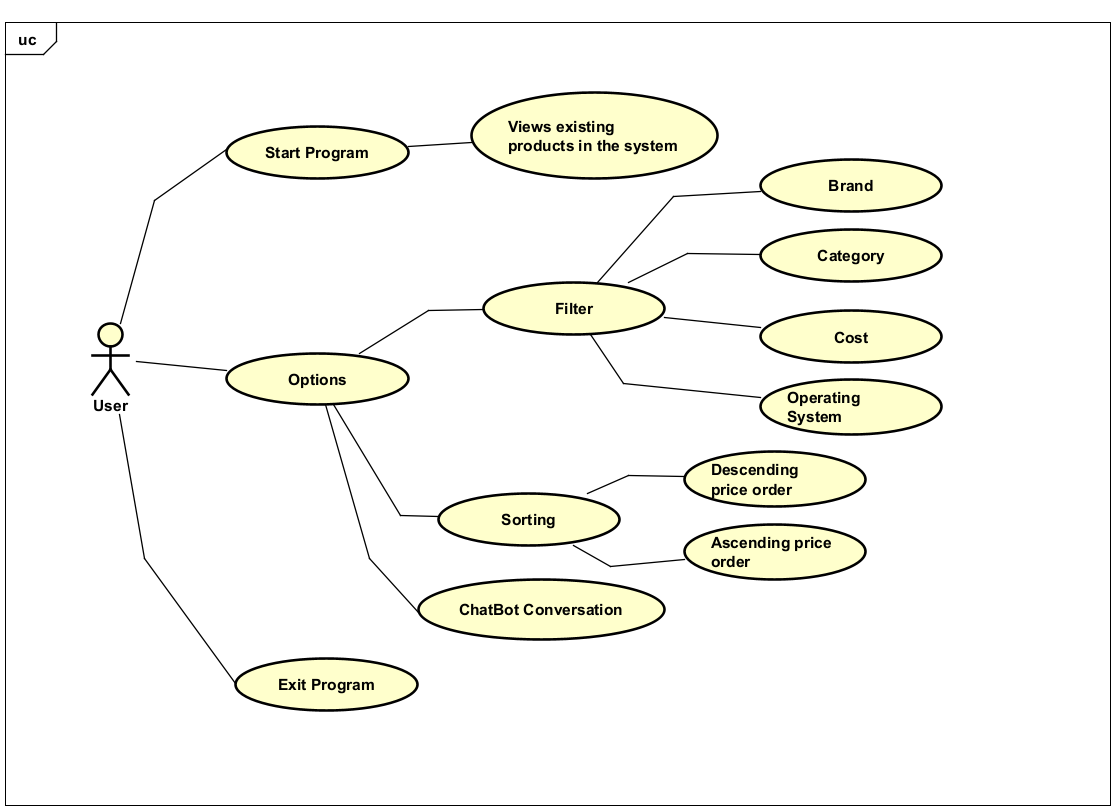
\includegraphics[width=0.9\textwidth]{UseCase.png} % Replace with actual diagram
    % \caption{Use Case Diagram} % Add caption if needed
\end{figure}

\subsection{Use Case Description}
\subsubsection{Actors}
\begin{itemize}
    \item \textbf{User:} The person interacting with the system to search for and receive recommendations on laptops.
\end{itemize}

\subsubsection{Use Cases}
\begin{itemize}
    \item \textbf{Start Program:} The user initiates the system (The entry point for all further interactions).
    \begin{itemize}
        \item \textit{Views Existing Products in the System:} The user can browse all available laptop products stored in the system.
    \end{itemize}
    \item \textbf{Options:} Once the program starts, the user accesses different options that include filtering, sorting, and engaging in chatbot conversation.
    \begin{itemize}
        \item \textit{Filter:} Allows the user to narrow down the list of products based on specific criteria:
        \begin{itemize}
            \item \textbf{Brand:} Filters laptops by manufacturer (e.g., Dell, HP, Apple).
            \item \textbf{Category:} Filters by use case or type (e.g., gaming, ultrabook, business).
            \item \textbf{Cost:} Filters by price range.
            \item \textbf{Operating System:} Filters based on OS (e.g., Windows, macOS, Linux).
        \end{itemize}
        \item \textit{Sorting:} The user can sort the displayed products by price:
        \begin{itemize}
            \item \textbf{Descending Price Order:} Highest price to lowest.
            \item \textbf{Ascending Price Order:} Lowest price to highest.
        \end{itemize}
        \item \textit{ChatBot Conversation:} This use case allows the user to engage with a chatbot powered by a large language model (LLM) to receive personalized recommendations or ask questions in natural language.
    \end{itemize}
    \item \textbf{Exit Program:} Ends the session and closes the system.
\end{itemize}

\section{Architecture}

\subsection*{Package Diagram}

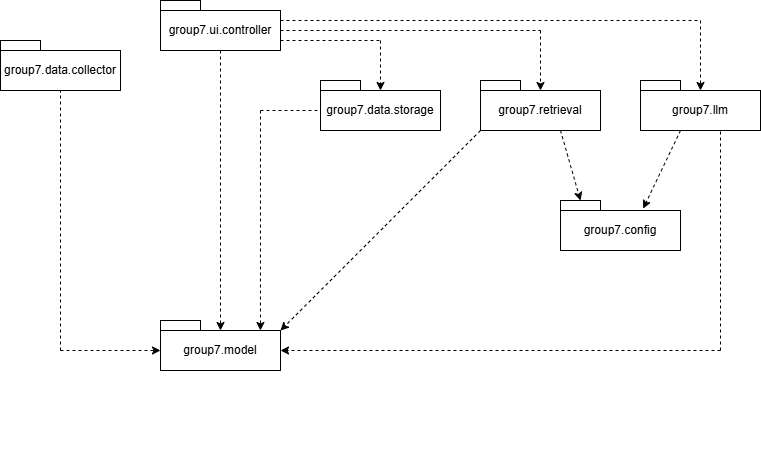
\includegraphics[width=\textwidth, keepaspectratio]{package.png}

\newpage
\subsection{Package model (\texttt{group7.model})}
\noindent
\begin{figure}[h!]
    \centering
    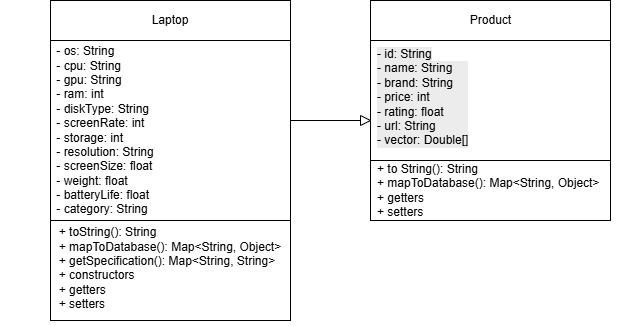
\includegraphics[width=\textwidth, keepaspectratio]{model.png} % Replace with actual diagram
\end{figure}

The \texttt{group7.model} package is responsible for defining the core data structures, or "models," that represent the entities within the application. It establishes a clear hierarchy for product-related data, facilitating organized data management, reusability, and extensibility.

\subsubsection{Class \texttt{Product}}
The \texttt{Product} class serves as a base (or parent) class for all types of products in the system. It encapsulates common attributes and functionalities shared across different product categories.
\begin{itemize}
    \item \textbf{Attributes (Fields):}
    \begin{itemize}
        \item \texttt{id: String} - A unique identifier for the product.
        \item \texttt{name: String} - The display name of the product.
        \item \texttt{brand: String} - The manufacturer or brand of the product.
        \item \texttt{price: int} - The price of the product (integer representation).
        \item \texttt{rating: float} - The customer rating of the product.
        \item \texttt{url: String} - A URL link to the product's page or image.
        \item \texttt{vector: double[]} - A numerical vector representation (embedding) of the product, crucial for similarity searches and recommendation features.
    \end{itemize}
    \item \textbf{Methods:}
    \begin{itemize}
        \item \texttt{Product()} - Default constructor.
        \item \texttt{Product(id, name, brand, price, rating, url)} - Parameterized constructor to initialize common product attributes (note: vector is set separately).
        \item \texttt{mapToDatabase(): Map<String, Object>} - Likely returns a map representation of the product's data, suitable for database persistence or data transfer.
        \item \texttt{toString(): String} - Provides a string representation of the product, often used for logging or basic display.
        \item Standard getter and setter methods for all its attributes (e.g., \texttt{getId()}, \texttt{setId(String id)}, \texttt{getVector()}, \texttt{setVector(double[] vector)}, etc.).
    \end{itemize}
\end{itemize}
The \texttt{Product} class forms the foundation for a polymorphic design, allowing different product types to be treated uniformly where appropriate, while also providing a common interface for accessing shared data.

\subsubsection{Class \texttt{Laptop}}
The \texttt{Laptop} class is a specialized type of \texttt{Product}, inheriting all attributes and methods from the \texttt{Product} class and adding specific details relevant to laptops.
\begin{itemize}
    \item \textbf{Inheritance:} \texttt{Laptop} extends \texttt{Product}.
    \item \textbf{Attributes (Fields) - Specific to Laptop:}
    \begin{itemize}
        \item \texttt{os: String} - Operating System (e.g., "Windows 11", "macOS").
        \item \texttt{cpu: String} - Central Processing Unit (e.g., "Intel Core i7").
        \item \texttt{gpu: String} - Graphics Processing Unit (e.g., "NVIDIA GeForce RTX 3060").
        \item \texttt{ram: int} - Random Access Memory in GB (e.g., 16).
        \item \texttt{diskType: String} - Type of storage disk (e.g., "SSD", "HDD").
        \item \texttt{screenRate: int} - Screen refresh rate in Hz (e.g., 120).
        \item \texttt{storage: int} - Storage capacity in GB or TB (e.g., 512 for 512GB).
        \item \texttt{resolution: String} - Screen resolution (e.g., "1920x1080").
        \item \texttt{screenSize: float} - Diagonal screen size in inches (e.g., 15.6).
        \item \texttt{weight: float} - Weight of the laptop in kg or lbs.
        \item \texttt{batteryLife: float} - Estimated battery life in hours.
        \item \texttt{category: String} - Specific laptop category (e.g., "Gaming", "Ultrabook", "Business").
    \end{itemize}
    \item \textbf{Methods:}
    \begin{itemize}
        \item \texttt{Laptop()} - Default constructor.
        \item \texttt{Laptop(id, name, brand, category, os, price, ..., url)} - A comprehensive parameterized constructor that initializes all attributes from both \texttt{Product} and \texttt{Laptop}.
        \item \texttt{getSpecification(): Map<String, String>} - Returns a map of the laptop's detailed technical specifications, likely used for display on product detail pages.
        \item \texttt{toString(): String} - Overrides the \texttt{Product.toString()} method to include laptop-specific information in its string representation.
        \item \texttt{mapToDatabase(): Map<String, Object>} - Overrides the \texttt{Product.mapToDatabase()} method to include laptop-specific data when preparing data for storage.
        \item Standard getter and setter methods for all its specific attributes (e.g., \texttt{getOs()}, \texttt{setOs(String os)}, \texttt{getCpu()}, etc.).
    \end{itemize}
\end{itemize}
\textbf{OOP Techniques Used:}
\begin{itemize}
    \item The relationship between \texttt{Laptop} and \texttt{Product} is a classic example of \textbf{Inheritance} (an "is-a" relationship), promoting code reuse and allowing for flexible handling of different product types.
    \item This structure makes it easy to add other product types in the future (e.g., \texttt{Smartphone}, \texttt{Tablet}) by having them also extend the \texttt{Product} class.
\end{itemize}

\subsection{Package ui (User Interface \texttt{group7.ui})}

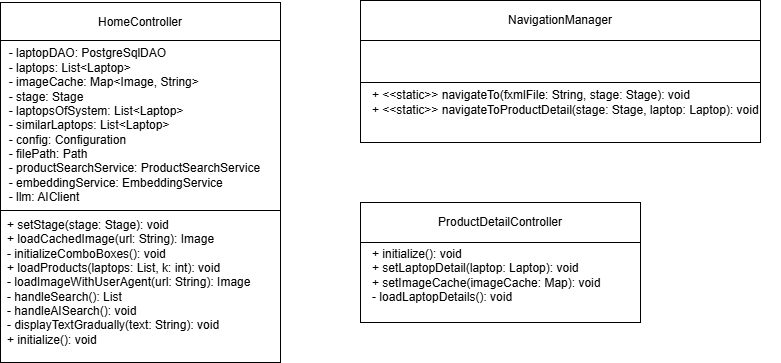
\includegraphics[width=\textwidth, keepaspectratio]{ui.png} % Replace with actual diagram

\subsubsection{Overview}
Create an interactive interface for the user, including components like buttons, search bars, images, etc. This links to corresponding services to provide functionality to the user.
\begin{itemize}
    \item \textbf{Main components of UI code:} Code originating from the \texttt{Main.java} file; FXML files for building the interface; Controller classes linked to their respective FXML files.
\end{itemize}

\subsubsection{Process}
\begin{itemize}
    \item Research
    \item Wireframing \& Prototyping
    \item Testing
\end{itemize}

\subsubsection{UI Design}
% This section seems to be a heading for the next part

\subsubsection{\texttt{HomeController.java} Class}
\begin{itemize}
    \item \textbf{Purpose:} This class controls "\texttt{Home.fxml}" - the application's main screen. It allows the user to:
    \begin{itemize}
        \item View a list of laptop products displayed as product cards.
        \item Search for laptops by criteria: brand, category, operating system, or keyword.
        \item Switch to the chat screen with the chatbot when the chat button is pressed.
    \end{itemize}
    \item \textbf{Function Structure:}
    \begin{itemize}
        \item \texttt{initialize()}: Controller initialization function, called automatically when FXML is loaded.
        \subitem \textit{Steps to build the function:}
        \begin{itemize}
            \item Initialize DAO (Data Access Object) to connect to the PostgreSQL database.
            \item Retrieve all laptop data from the database.
            \item Create and display product cards on the \texttt{GridPane}.
            \item Set up listeners for the search box and \texttt{ComboBoxes}.
            \item Set up the event for the chat button.
            \item Initialize values for \texttt{ComboBoxes}.
        \end{itemize}
        \item \texttt{setStage(Stage stage)}: Sets the current stage (window) for the controller.
        \subitem \textit{Steps to build the function:}
        \begin{itemize}
            \item Store a reference to the stage to enable navigation between scenes.
        \end{itemize}
        \item \texttt{initializeComboBoxes()}: Initializes values for the product filter \texttt{ComboBoxes}.
        \subitem \textit{Steps to build the function:}
        \begin{itemize}
            \item Add selection values for the brand \texttt{ComboBox}.
            \item Add selection values for the category \texttt{ComboBox}.
            \item Add selection values for the operating system \texttt{ComboBox}.
            \item Set the default value to "All" for all \texttt{ComboBoxes}.
        \end{itemize}
        \item \texttt{handleSearch()}: Handles product search and filtering based on criteria.
        \subitem \textit{Steps to build the function:}
        \begin{itemize}
            \item Retrieve all products from the database.
            \item Get filter values from \texttt{ComboBoxes} and the search box.
            \item Filter products by brand if selected.
            \item Filter products by category if selected.
            \item Filter products by operating system if selected.
            \item Reload the list of filtered products.
        \end{itemize}
        \item \texttt{switchToChatbot(MouseEvent event)}: Handles the event to switch to the chatbot screen.
        \subitem \textit{Steps to build the function:}
        \begin{itemize}
            \item Currently only prints a console message, can be expanded to switch scenes later.
        \end{itemize}
    \end{itemize}
\end{itemize}

\subsubsection{\texttt{NavigationManager.java} Class}
\begin{itemize}
    \item \textbf{Purpose:} This class acts as a navigation manager within the application. It allows:
    \begin{itemize}
        \item Switching between different screens (scenes) in the application.
        \item Handling the loading of FXML files and scene switching.
        \item Passing data between screens during transitions.
    \end{itemize}
    \item \textbf{Function Structure:}
    \begin{itemize}
        \item \texttt{navigateTo(String fxmlFile, Stage stage)}: Navigates to a new screen specified by the FXML file.
        \subitem \textit{Steps to build the function:}
        \begin{itemize}
            \item Create an \texttt{FXMLLoader} to load the FXML file from the view directory.
            \item Create a new \texttt{Scene} from the loaded FXML.
            \item Set the new \texttt{Scene} for the current \texttt{Stage}.
            \item Display the \texttt{Stage} with the new \texttt{Scene}.
        \end{itemize}
        \item \texttt{navigateToProductDetail(Stage stage, String laptopId)}: Navigates to the product detail screen with a specific laptop ID.
        \subitem \textit{Steps to build the function:}
        \begin{itemize}
            \item Create an \texttt{FXMLLoader} to load the \texttt{ProductDetail.fxml} file.
            \item Create a new \texttt{Scene} from the loaded FXML.
            \item Get the controller from the \texttt{FXMLLoader}.
            \item Pass the \texttt{laptopId} to the controller of the product detail screen.
            \item Set the new \texttt{Scene} for the current \texttt{Stage}.
            \item Display the \texttt{Stage} with the new \texttt{Scene}.
        \end{itemize}
    \end{itemize}
\end{itemize}

\subsubsection{\texttt{ProductDetailController.java} Class}
\begin{itemize}
    \item \textbf{Purpose:} This class controls "\texttt{ProductDetail.fxml}" - the laptop product detail screen. It allows the user to:
    \begin{itemize}
        \item Display full detailed information of a specific laptop product.
        \item Handle the event to return to the main screen (\texttt{Home.fxml}).
        \item Load and display product data based on the passed ID.
    \end{itemize}
    \item \textbf{Function Structure:}
    \begin{itemize}
        \item \texttt{initialize()}: Controller initialization function, called automatically when FXML is loaded.
        \subitem \textit{Steps to build the function:}
        \begin{itemize}
            \item Initialize DAO (Data Access Object) to connect to the PostgreSQL database.
            \item Set up the event for the back button to return to the main screen.
        \end{itemize}
        \item \texttt{setStage(Stage stage)}: Sets the current stage (window) for the controller.
        \subitem \textit{Steps to build the function:}
        \begin{itemize}
            \item Store a reference to the stage to enable navigation between scenes.
        \end{itemize}
        \item \texttt{setLaptopId(String laptopId)}: Sets the laptop ID and loads detailed information.
        \subitem \textit{Steps to build the function:}
        \begin{itemize}
            \item Store the \texttt{laptopId} in a member variable.
            \item Call the \texttt{loadLaptopDetails()} function to load product information.
        \end{itemize}
        \item \texttt{loadLaptopDetails()}: Loads and displays detailed information of the laptop.
        \subitem \textit{Steps to build the function:}
        \begin{itemize}
            \item Retrieve all products from the database.
            \item Find the product with the ID matching \texttt{laptopId}.
            \item If found, display all product information on corresponding Labels, format numerical values (price, rating, screen size, etc.), load and display the product image from URL.
            \item If not found, display a "Product not found" message.
        \end{itemize}
    \end{itemize}
\end{itemize}

\subsubsection{FXML Files}
\begin{itemize}
    \item \textbf{Purpose:} These files define the user interface structure and appearance.
    \begin{itemize}
        \item "\texttt{Chat.fxml}": User interface for the chatbot conversation screen, including an area to display chatbot responses.
        \item "\texttt{Home.fxml}": User interface for the application's main screen, including: a header with a background image and search bar, a product filter area, and an area to display the product list in a grid.
        \item "\texttt{ProductCard.fxml}": Interface for a single product card (laptop), including: product image, product name, product price, view details button.
        \item "\texttt{ProductDetail.fxml}": Interface for the laptop product detail screen, including: product image, basic information (name, rating, price), detailed product description, full technical specifications.
    \end{itemize}
    \item \textbf{Structure:} FXML files use common and diverse UI components such as:
    \begin{itemize}
        \item \textit{Layout Containers:}
        \begin{itemize}
            \item \texttt{VBox} (vertical layout)
            \item \texttt{HBox} (horizontal layout)
            \item \texttt{GridPane} (grid layout)
            \item \texttt{StackPane} (stacking layers)
        \end{itemize}
        \item \textit{Controls:}
        \begin{itemize}
            \item \texttt{Label}: Displays text
            \item \texttt{Button}: Interactive button
            \item \texttt{TextField}: Input field
            \item \texttt{ComboBox}: Dropdown for selecting values
            \item \texttt{TextArea}: Displays long text
        \end{itemize}
        \item \textit{Media:}
        \begin{itemize}
            \item \texttt{ImageView}: Displays images
            \item \texttt{Image}: Image source
        \end{itemize}
        \item \textit{Utilities:}
        \begin{itemize}
            \item \texttt{ScrollPane}: Creates a scrollable frame
            \item \texttt{FXCollections}: Creates lists for \texttt{ComboBoxes}
        \end{itemize}
    \end{itemize}
\end{itemize}

\subsection{Package data (\texttt{group7.data})}
\noindent 
\begin{figure}[h!]
    \centering
    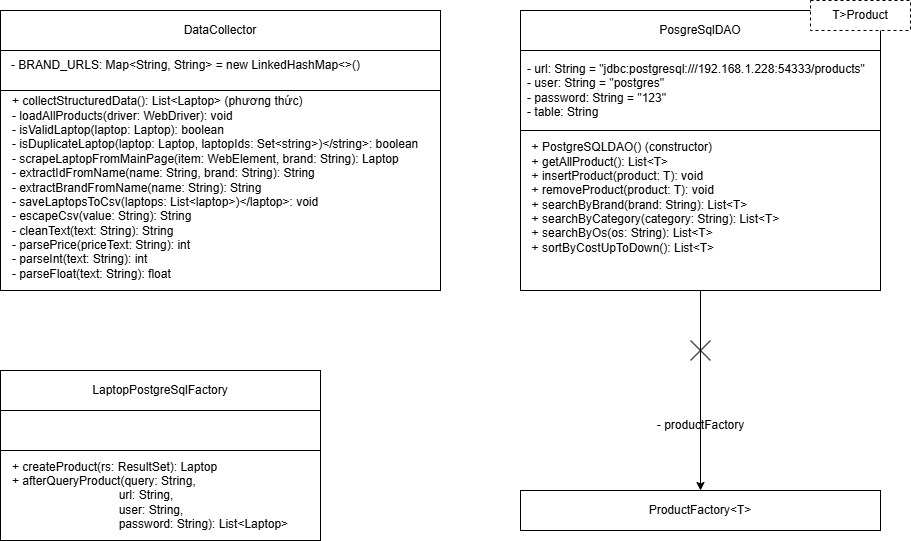
\includegraphics[width=\textwidth, keepaspectratio]{data.png} % Replace with actual diagram
\end{figure}

\subsubsection{Package collector (\texttt{group7.data.collector} (\texttt{DataCollector.java}))}
\begin{itemize}
    \item \textbf{Main Idea:} The \texttt{DataCollector} class is designed to collect information about laptop products from an online retail website (\url{https://www.thegioididong.com}) by using Selenium WebDriver to automate web browsing, extract product information, and store it in a CSV file. The data is organized into Laptop objects to ensure structure and ease of use in other applications.
    \item \textbf{Class Operation:}
    \begin{enumerate}
        \item \textit{Initialization and Configuration:}
        \begin{itemize}
            \item Uses \texttt{LinkedHashMap} to store a list of laptop brands and their corresponding URLs (GAMING, AI, MACBOOK, HP, ASUS, DELL, ACER, LENOVO, MSI).
            \item Configures \texttt{ChromeDriver} in headless mode (no GUI displayed) to optimize performance and automatically downloads the appropriate driver using \texttt{WebDriverManager}.
        \end{itemize}
        \item \textit{Data Collection (\texttt{collectStructuredData}):}
        \begin{itemize}
            \item Iterates through each brand and URL in \texttt{BRAND\_URLS}.
            \item Opens the webpage using WebDriver, scrolls the page to load all products (\texttt{loadAllProducts}).
            \item Finds all product elements (\texttt{li.item}) on the page and extracts detailed information using the \texttt{scrapeLaptopFromMainPage} method.
            \item Checks for validity and duplication of laptops before adding them to the laptops list.
            \item Limits the number of laptops collected to a maximum of 360 (\texttt{MAX\_LAPTOPS}).
        \end{itemize}
        \item \textit{Information Extraction (\texttt{scrapeLaptopFromMainPage}):}
        \begin{itemize}
            \item Retrieves information from HTML elements (name, price, rating, image, RAM, storage capacity, CPU, GPU, screen size, resolution, etc.).
            \item Processes raw data using utility methods (\texttt{cleanText}, \texttt{parsePrice}, \texttt{parseInt}, \texttt{parseFloat}) to clean and convert formats.
            \item Determines the actual brand and category based on the product name or provided brand.
        \end{itemize}
        \item \textit{Data Storage (\texttt{saveLaptopsToCsv}):}
        \begin{itemize}
            \item Saves the list of laptops to a CSV file with UTF-8 encoding, adding a BOM to support displaying Vietnamese characters.
            \item Each laptop is saved as a row with information fields separated by commas, ensuring special characters are handled by the \texttt{escapeCsv} method.
        \end{itemize}
        \item \textit{Resource Management:}
        \begin{itemize}
            \item Closes the browser (\texttt{driver.quit()}) after data collection to free up resources.
        \end{itemize}
    \end{enumerate}
    \item \textbf{Advantages of the class:}
    \begin{itemize}
        \item \textit{Efficient Automation:} Uses Selenium WebDriver to automate web browsing and scrolling, helping to load all products without manual intervention. Headless mode increases performance and reduces resource usage.
        \item \textit{Clear Data Structure:} Data is organized into \texttt{Laptop} objects, making it easy to reuse and integrate into other systems. Uses \texttt{LinkedHashMap} to maintain brand order and \texttt{HashSet} for quick duplicate checking.
        \item \textit{Good Error Handling:} Handles exceptions at multiple levels (URL connection, product processing, HTML element access), ensuring the program does not terminate unexpectedly. Checks for validity (\texttt{isValidLaptop}) and duplication (\texttt{isDuplicateLaptop}) to ensure data quality.
        \item \textit{Easy Maintenance and Expansion:} Code is divided into small methods with specific functions, making it easy to modify or add features. URLs and brands are stored in \texttt{BRAND\_URLS}, easy to update or supplement.
        \item \textit{Optimized Performance:} Uses \texttt{implicitlyWait} to reduce waiting time when finding elements. Measures the processing time for each product to monitor performance.
    \end{itemize}
    \item \textbf{OOP Techniques Used:}
    \begin{itemize}
        \item \textit{Encapsulation:} Attributes like \texttt{BRAND\_URLS} are declared as \texttt{private static final}, ensuring they are not modified from outside. Helper methods (\texttt{cleanText}, \texttt{parsePrice}, etc.) are defined as \texttt{private} for internal use within the class.
        \item \textit{Abstraction:} The \texttt{DataCollector} class provides a simple interface (\texttt{collectStructuredData}) to collect data without the user needing to know the internal implementation details (Selenium, scrolling, HTML processing).
        \item \textit{Reusability:} Utility methods (\texttt{cleanText}, \texttt{parsePrice}, \texttt{parseInt}, \texttt{parseFloat}) can be reused in other classes or projects. The \texttt{Laptop} data structure can be integrated into other systems (e.g., data analysis, UI display).
    \end{itemize}
\end{itemize}

\subsubsection{Package storage(\texttt{group7.data.storage})}
\textbf{Interface \texttt{ProductFactory<T>}}
\begin{itemize}
    \item Has two functions: the first function returns a product of type T from the query result in the database.
    \item The second function returns a list of products of type T after passing a query to the database with a URL, user, and password.
    \item Implemented by the abstract class \texttt{SqlFactory()}.
\end{itemize}
\textbf{Class \texttt{LaptopPostgreSqlFactory} implements \texttt{ProductFactory<Laptop>}}
\begin{itemize}
    \item The \texttt{LaptopPostgreSqlFactory} class is used to create laptop objects from a query.
    \item If other product types or database types need to be added, similar Factory classes inheriting \texttt{SqlFactory} would need to be written.
    \item For example, \texttt{PhoneMySqlFactory}.
\end{itemize}
\textbf{Class \texttt{PostgreSqlDAO<T extends Product>}}
\begin{itemize}
    \item Used to access the database and handle functions as defined by \texttt{ProductDAO<>}.
    \item Uses generic programming to comfortably switch between product types available in the PostgreSQL database.
    \item If we want to use another database type, we just need to write another DAO class. In \texttt{PostgreSqlDAO}, we have an attribute \texttt{ProductFactory<T> productFactory}, which helps separate logic: \texttt{postgresqlDAO} only needs to handle database connection and queries, while the factory handles data conversion.
    \item Additionally, it helps with reusability. For instance, if working with laptops, I would assign the \texttt{productFactory} attribute as \texttt{new LaptopPostgreSqlFactory()}, T := \texttt{Laptop}. Or if working with phones, then \texttt{productFactory = new PhonePostgreSqlFactory()}.
    \item In general, when wanting to work with a specific database type and product type, one only needs to care about the type of T, the table name of the product, and the \texttt{productFactory}.
    \item For example, for laptops: \texttt{ProductDAO<Laptop> admin = new PostgreSqlDAO<Laptop>("laptop", new LaptopPostgreSqlFactory());}. We have created an admin reference that can perform all functions in the \texttt{ProductDAO<>} interface.
    \item If we want to switch to handling Phones, we only need to change it to \texttt{ProductDAO<Phone> admin = new PostgreSqlDAO<Phone>("phone", new PhonePostgreSqlFactory());}.
\end{itemize}

\subsection{Package retrieval (\texttt{group7.retrieval})}

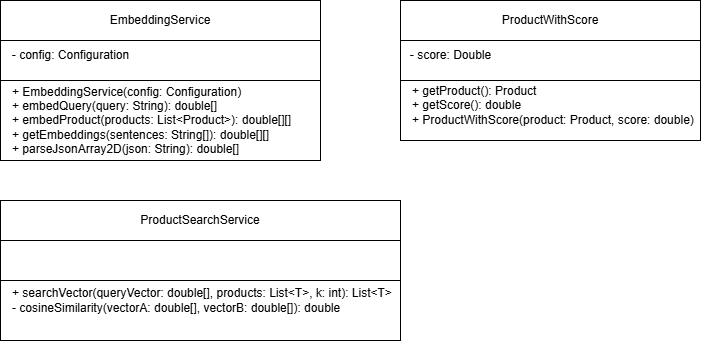
\includegraphics[width=\textwidth, keepaspectratio]{retrieval.png}

Package \texttt{group7.retrieval} is designed to handle tasks related to information retrieval in the system, specifically searching for products based on vector embeddings and calculating similarity. The system's recommendation model works by representing products and user queries as numerical vectors and calculating cosine similarity, then providing suggestions to the user.

\subsubsection{Class \texttt{ProductWithScore}}
\begin{itemize}
    \item The \texttt{ProductWithScore} class in package \texttt{group7.retrieval} is designed to encapsulate a \texttt{Product} object along with its corresponding score, used in search and product ranking tasks.
    \item This class combines a \texttt{Product} object with a score value, typically representing the relevance of the product to a search query.
    \item The \texttt{product} attribute is marked as \texttt{final}, ensuring that the \texttt{Product} object cannot be changed after initialization, increasing safety and consistency.
    \item \texttt{ProductWithScore} can contain any object belonging to the \texttt{Product} class or its subclasses, serving the purpose of reusability for this class in the future when the system expands to products beyond Laptops.
\end{itemize}

\subsubsection{Class \texttt{ProductSearchService}}
The \texttt{ProductSearchService} class in package \texttt{group7.retrieval} uses the \texttt{cosineSimilarity} function to compare the query vector with product vectors, rank products by similarity, and return a list of the k most suitable products.
The \texttt{searchVector} method receives the following inputs:
\begin{itemize}
    \item \texttt{queryVector}: Vector representing the search query (usually created by \texttt{EmbeddingService}).
    \item \texttt{products}: List of products (of type \texttt{T extends Product}) to search.
    \item \texttt{k}: Maximum number of products to return.
\end{itemize}
This method returns a list of k products with the highest similarity to \texttt{queryVector}.\\
\textbf{Operating Principle:}
\begin{itemize}
    \item This method creates a list \texttt{scoredProducts} (of type \texttt{List<ProductWithScore>}) to store products along with their similarity scores. For each product in \texttt{products}, its vector is retrieved, and its similarity to \texttt{queryVector} is calculated using the \texttt{cosineSimilarity} function. A \texttt{ProductWithScore} object is created and stored in the \texttt{scoredProducts} list for sorting.
    \item The \texttt{scoredProducts} list is sorted by score in descending order (using \texttt{sort} with \texttt{Double.compare}), then the first k products are taken from the list, cast to type T, and added to the results list to be returned.
    \item This method uses a generic type (\texttt{<T extends Product>}) for generalization. T is a generic type constrained by \texttt{extends Product}, meaning T must be a specific class or a subclass of the \texttt{Product} class (from package \texttt{group7.model}). For example, T can be \texttt{Laptop}, \texttt{Smartphone}, \texttt{Tablet}, or any class that inherits from \texttt{Product}.
\end{itemize}
\textbf{Benefits:}
\begin{itemize}
    \item \textit{Flexibility:} The method can handle various product types (laptop, smartphone, etc.) without requiring separate code for each type.
    \item \textit{Separation of search logic and product representation:} The method is not concerned with the specific details of the product (like attributes of \texttt{Laptop} or \texttt{Smartphone}). It only needs a query vector (\texttt{queryVector}) and a list of products with a \texttt{getVector()} method that returns an embedding vector.
    \item \textit{Type safety:} Generic types ensure that the input list (\texttt{products}) and the result list (\texttt{List<T>}) have the same type T, reducing the risk of unsafe type casting errors at runtime.
    \item \textit{Code reusability:} A single method can be used for multiple product types, instead of writing separate methods for each.
\end{itemize}
The \texttt{cosineSimilarity} function calculates the cosine similarity between two vectors, returning a value in the range [-1, 1]:
\[ \text{cosineSimilarity} = \frac{\text{dotProduct}}{\sqrt{\text{normA}} \cdot \sqrt{\text{normB}}} \]

\subsubsection{Class \texttt{EmbeddingService}}
\begin{itemize}
    \item The \texttt{EmbeddingService} class in package \texttt{group7.retrieval} is designed to create vector embeddings for queries and products, using an external API to convert text into numerical vectors. This class can handle any product type belonging to the \texttt{Product} class or its subclasses, as long as the product has a \texttt{toString()} method to represent it as text.
    \item \texttt{private final Configuration config}: Stores the configuration object (\texttt{Configuration}), providing information such as the API embedding URL (\texttt{config.getApiUrl()}). Using \texttt{final} ensures immutability, increasing safety and consistency.
    \item The \texttt{embedQuery} method converts a text query into an embedding vector. This method provides the \texttt{query vector} to \texttt{ProductSearchService} for comparison with product vectors.
    \item The \texttt{embedProducts} method converts a list of products into embedding vectors.
    \item Using \texttt{List<? extends Product>} instead of \texttt{List<Product>} allows handling any list of products belonging to the \texttt{Product} class or its subclasses (like \texttt{Laptop}, \texttt{Smartphone}, etc.).
    \item This makes the method flexible, applicable to various product types without code changes.
    \item The \texttt{getEmbeddings} method sends an HTTP POST request to the API to get embeddings for a list of sentences.
\end{itemize}
\textbf{How it works:}
\begin{enumerate}
    \item \textit{Build JSON:}
    \begin{itemize}
        \item Create a JSON string with the format \texttt{\{"sentences": ["sentence1", "sentence2", ...]\}}.
        \item Escape """ characters in sentences to ensure valid JSON.
    \end{itemize}
    \item \textit{Send HTTP request:}
    \begin{itemize}
        \item Open a connection to the URL from \texttt{config.getApiUrl()}.
        \item Set the method to POST, and headers \texttt{Content-Type} and \texttt{Accept} to \texttt{application/json}.
        \item Send the JSON string via \texttt{OutputStream}.
    \end{itemize}
    \item \textit{Receive and process response:}
    \begin{itemize}
        \item Read the response from \texttt{InputStream} and save it to a \texttt{StringBuilder}.
        \item Call \texttt{parseJsonArray2D} to convert JSON into a \texttt{double[][]} array.
    \end{itemize}
    \item \textit{Disconnect:} Close the HTTP connection after completion.
\end{enumerate}
The \texttt{parseJsonArray2D} method uses the Gson library to parse JSON into a \texttt{double[][]} array.
The \texttt{EmbeddingService} class is designed with high generalization, demonstrated by:
\begin{itemize}
    \item \textit{Support for multiple product types.} The \texttt{embedProducts} method uses \texttt{List<? extends Product>}, allowing it to process any list of products that are subtypes of \texttt{Product}. This ensures the class can work with any product type, as long as they have a valid \texttt{toString()} method.
    \item \textit{Configuration separation.} Using \texttt{Configuration} to get \texttt{getApiUrl()} helps the class not depend on a specific URL. This allows easy API or configuration changes without modifying the code.
    \item \textit{Independence from product details.} The class only requires products to provide text via \texttt{toString()}. This makes \texttt{EmbeddingService} unaware of the detailed structure of \texttt{Product} classes or their subclasses, increasing abstraction.
    \item \textit{Batch processing support:} The \texttt{getEmbeddings} method accepts a \texttt{String[]} array, allowing embeddings for multiple sentences (queries or products) to be created simultaneously, optimizing communication with the API.
\end{itemize}

\subsection{Package llm (\texttt{group7.llm})}

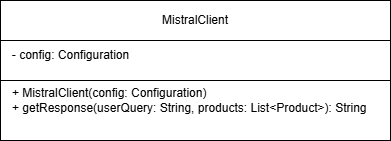
\includegraphics[width=0.7\textwidth, keepaspectratio, center]{llm.png} % Replace with actual diagram

Package \texttt{group7.llm} is designed to integrate and use Large Language Models (LLMs) to provide responses based on artificial intelligence, especially in the context of product consultation.

\subsubsection*{Class \texttt{MistralClient}}
\begin{itemize}
    \item This class implements the \texttt{AIClient} interface and performs specific tasks to interact with the Mistral AI API.
    \item \textbf{Constructor:} Receives a \texttt{Configuration} object to get configuration information (API URL, API key), ensuring flexibility and avoiding hard-coding.
    \item \textbf{Method \texttt{getResponse}:} Processes the user query and product list, calls the Mistral API to generate a consultation response.
\end{itemize}
\textbf{How it works:}
\begin{itemize}
    \item \textit{Build prompt:} Converts the product list into a text string by calling \texttt{toString()} on each product. Creates a prompt including:
    \begin{itemize}
        \item User query (\texttt{userQuery}).
        \item Product list.
        \item Request for LLM to suggest the 5 most suitable products and explain why.
    \end{itemize}
    \item \textit{Create JSON request:} Uses the \texttt{org.json} library to build JSON with:
    \begin{itemize}
        \item A system message defining the LLM's role as a "useful product consultant".
        \item A user message containing the prompt.
        \item Parameters like model (Mistral AI model) and temperature (creativity level, default 0.7).
    \end{itemize}
    \item \textit{Send HTTP request:} Uses \texttt{HttpClient} to send a POST request to the Mistral API with:
    \begin{itemize}
        \item URL from \texttt{config.getApiEndpoint()}.
        \item Authorization header with API key from \texttt{config.getApiKey()}.
        \item Body as JSON string.
    \end{itemize}
    \item \textit{Process response:} Parses the JSON response to get content from the \texttt{choices[0].message.content} field. Returns the response content as a string.
    \item \textit{Error handling:} Catches exceptions and returns a default error message: "Error calling Mistral API".
\end{itemize}
\textbf{Generalization Features:}
\begin{itemize}
    \item \textit{Support for multiple product types:} Uses \texttt{List<? extends Product>} to allow processing any list of products belonging to the \texttt{Product} class or its subclasses.
    \item \textit{Flexible integration:} Relies on \texttt{Configuration} to get URL and API key, making it easy to switch to another API or change configuration.
    \item \textit{Extensibility:} Since it implements the \texttt{AIClient} interface, \texttt{MistralClient} can be replaced by other implementations without affecting the calling code.
\end{itemize}

\subsection{Package config (\texttt{group7.config})}

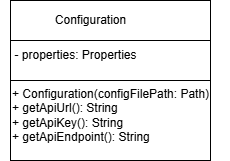
\includegraphics[width=0.5\textwidth, keepaspectratio]{config.png} % This assumes the provided image is named configuration.png

Package \texttt{group7.config} is responsible for managing application settings, such as API credentials and service URLs. Its main goal is to abstract configuration details away from the core application logic, allowing for easy updates and maintenance without modifying the source code.

\subsubsection*{Class \texttt{Configuration}}
\begin{itemize}
    \item This class is designed to load and provide access to configuration properties from an external file.
    \item \textbf{Constructor:} Takes a \texttt{Path} object pointing to the configuration file (e.g., config.properties) and initializes the class by loading the properties from this file.
    \item \textbf{Methods \texttt{getApiUrl}, \texttt{getApiKey}, \texttt{getApiEndpoint}:} These methods provide access to specific configuration values (API URL, key, and endpoint) stored in the properties file. They retrieve the corresponding value for a predefined key (e.g., api.url, api.key).
\end{itemize}

\textbf{How it works:}
\begin{itemize}
    \item \textit{Initialization:} An instance of Configuration is created by passing the path to a .properties file.
    \item \textit{Load Properties:} The constructor uses a FileInputStream to open the specified file. It then initializes a java.util.Properties object and calls its load() method, which parses the input stream from the file. This populates the internal properties object with key-value pairs defined in the file.
    \item \textit{Data Retrieval:} When a getter method like getApiKey() is called, it uses the getProperty(String key) method of the Properties object to look up and return the value associated with the corresponding key (e.g., "api.key").
    \item \textit{Error Handling:} The class includes error handling to manage IOException (e.g., if the configuration file is not found or cannot be read), ensuring the application fails gracefully or reports a clear error.
\end{itemize}

\textbf{Generalization Features:}
\begin{itemize}
    \item \textit{Separation of Concerns:} By isolating configuration in a separate class and file, the application's business logic (like in MistralClient) is decoupled from its configuration details. You can change the API key or URL without recompiling the code.
    \item \textit{Environment-Specific Configurations:} This design allows for easy management of different configurations for different environments (development, testing, production). A different .properties file can be supplied at runtime without any code changes.
    \item \textit{Easy to Extend:} To support new configuration parameters, one only needs to add a new key-value pair to the .properties file and a corresponding getter method in the Configuration class.
\end{itemize}

\section{Technology Stack}
\subsection{Frameworks \& Libraries}
\begin{enumerate}
    \item \textbf{Language:}
    \begin{itemize}
        \item \textbf{Java:} The primary programming language, evident from file names (\texttt{.java}), class structures, and mentioned libraries/frameworks.
    \end{itemize}
    \item \textbf{User Interface (UI):}
    \begin{itemize}
        \item \textbf{JavaFX:} Used for building the graphical user interface. Mentions include:
        \begin{itemize}
            \item FXML: For defining the UI structure declaratively.
            \item \texttt{Stage}, \texttt{Scene}: Core JavaFX windowing components.
            \item \texttt{ChatController}, \texttt{HomeController}, etc.: JavaFX controller classes.
            \item JavaFX UI Controls: \texttt{Button}, \texttt{Label}, \texttt{TextField}, \texttt{TextArea}, \texttt{ComboBox}, \texttt{ImageView}, \texttt{GridPane}, \texttt{VBox}, \texttt{HBox}, \texttt{StackPane}, \texttt{ScrollPane}.
            \item JavaFX Animation: \texttt{Timeline}, \texttt{KeyFrame} (for the typewriter effect).
        \end{itemize}
    \end{itemize}
    \item \textbf{Data Collection \& Web Interaction:}
    \begin{itemize}
        \item \textbf{Selenium WebDriver:} For automating web browser interaction to scrape laptop data from "\url{thegioididong.com}".
        \item \textbf{ChromeDriver:} Specific WebDriver implementation for Google Chrome.
        \item \textbf{WebDriverManager:} For automatically managing browser driver binaries.
    \end{itemize}
    \item \textbf{Database \& Data Persistence:}
    \begin{itemize}
        \item \textbf{PostgreSQL:} The relational database management system used for storing product data.
        \item \textbf{JDBC (Implicit):} Likely used for Java-to-PostgreSQL connectivity via the DAO layer, though not explicitly named, it's the standard.
        \item \textbf{CSV (Comma-Separated Values):} Used as a file format for storing the scraped laptop data (\texttt{saveLaptopsToCsv}).
    \end{itemize}
    \item \textbf{AI \& Machine Learning Integration:}
    \begin{itemize}
        \item \textbf{External Embedding API:} An unspecified external API is used to convert text (product descriptions, user queries) into numerical vector embeddings (via \texttt{EmbeddingService}).
        \item \textbf{Mistral AI API:} An LLM (Large Language Model) API used for the chatbot functionality to generate responses to user queries (\texttt{MistralClient} interacts with this).
        \item \textbf{JSON:} Used as the data interchange format for communicating with both the Embedding API and the Mistral AI API.
        \begin{itemize}
            \item \textbf{Gson library:} Explicitly mentioned for parsing JSON responses from the Embedding API.
            \item \textbf{org.json library:} Explicitly mentioned for constructing JSON requests for the Mistral AI API.
        \end{itemize}
    \end{itemize}
    \item \textbf{HTTP Communication:}
    \begin{itemize}
        \item \textbf{Java's built-in HTTP Client:} (\texttt{java.net.HttpURLConnection} or \texttt{java.net.http.HttpClient}) Used by \texttt{EmbeddingService} and \texttt{MistralClient} to make POST requests to external APIs.
    \end{itemize}
    \item \textbf{Configuration:}
    \begin{itemize}
        \item \textbf{\texttt{.properties} files:} Used for application configuration (e.g., \texttt{application.properties} storing API URLs, keys, database credentials).
    \end{itemize}
    \item \textbf{Design Patterns \& Architecture:}
    \begin{itemize}
        \item \textbf{Model-View-Controller (MVC) variant:} The separation of FXML (View), Controller classes, and Model classes (\texttt{Product}, \texttt{Laptop}) strongly suggests an MVC-like architecture.
        \item \textbf{Data Access Object (DAO):} \texttt{ProductDAO}, \texttt{PostgreSqlDAO} are used to abstract and encapsulate database interactions.
        \item \textbf{Factory Pattern / Abstract Factory Pattern:} \texttt{ProductFactory}, \texttt{SqlFactory} \\\texttt{LaptopPostgreSqlFactory} are used for creating product objects, decoupling client code from concrete class instantiation.
        \item \textbf{Service Layer:} Implied by classes like \texttt{EmbeddingService}, \texttt{ProductSearchService}, \texttt{AlClient}, which encapsulate specific business logic or external service interactions.
    \end{itemize}
    \item \textbf{Core Java Features:}
    \begin{itemize}
        \item \textbf{Java Collections Framework:} \texttt{List}, \texttt{Map}, \texttt{HashSet}, \texttt{LinkedHashMap} are used extensively for data management.
        \item \textbf{Generics:} Used heavily in DAO and Factory patterns (\texttt{<T extends Product>}) for type safety and reusability.
        \item \textbf{Object-Oriented Programming (OOP):} Encapsulation, Inheritance (\texttt{Laptop} extends \texttt{Product}), Polymorphism are fundamental to the design.
    \end{itemize}
\end{enumerate}

\subsection{Algorithms \& Techniques}
\begin{enumerate}
    \item \textbf{Information Retrieval \& Semantic Search:}
    \begin{itemize}
        \item \textbf{Vector Embeddings:} Textual descriptions of products and user queries are converted into dense vector representations. This allows for semantic understanding beyond simple keyword matching.
        \item \textbf{Cosine Similarity:} The mathematical measure used to determine the similarity between the query vector and product vectors. This is the core of the semantic search functionality (\texttt{ProductSearchService.cosineSimilarity}).
        \[ \text{cosineSimilarity} = \frac{\vec{A} \cdot \vec{B}}{||\vec{A}|| \cdot ||\vec{B}||} \]
        \item \textbf{Top-K Ranking/Retrieval:} After calculating similarities, the system ranks products and returns the top k most relevant ones to the user's query.
    \end{itemize}
    \item \textbf{AI Chatbot Interaction:}
    \begin{itemize}
        \item \textbf{Prompt Engineering:} The \texttt{MistralClient} constructs specific prompts (including user query, relevant product context, and instructions) to guide the LLM in generating useful and relevant responses.
        \item \textbf{LLM API Integration:} Sending structured requests to the Mistral AI API and parsing its JSON responses to extract the generated text.
    \end{itemize}
    \item \textbf{Web Scraping \& Data Extraction:}
    \begin{itemize}
        \item \textbf{Automated Browser Navigation:} Selenium is used to navigate web pages, scroll to load dynamic content (\texttt{loadAllProducts}).
        \item \textbf{HTML Element Selection \& Parsing:} Identifying and extracting data from specific HTML elements (e.g., \texttt{li.item}, product name, price, specs).
        \item \textbf{Data Cleaning \& Transformation:} Raw scraped data is processed (\texttt{cleanText}, \texttt{parsePrice}, \texttt{parseInt}, \texttt{parseFloat}) to ensure consistency and correct data types.
    \end{itemize}
    \item \textbf{User Interface Logic:}
    \begin{itemize}
        \item \textbf{Gradual Text Display (Typewriter Effect):} Implemented in \\\texttt{ChatController.displayTextGradually} using JavaFX \texttt{Timeline} and \texttt{KeyFrame} to enhance the user experience when displaying chatbot messages.
        \item \textbf{Client-Side Filtering:} The \texttt{HomeController} implements logic to filter the displayed product list based on user selections in \texttt{ComboBoxes} (brand, category, OS) and keyword search.
    \end{itemize}
    \item \textbf{Data Management \& Persistence:}
    \begin{itemize}
        \item \textbf{Object-Relational Mapping (Conceptual):} The DAO layer and methods like \texttt{mapToDatabase()} in model classes facilitate the translation of Java objects to a format suitable for storage in the PostgreSQL relational database.
        \item \textbf{CSV Data Serialization:} Converting lists of \texttt{Laptop} objects into a CSV file format for storage/export.
    \end{itemize}
\end{enumerate}

\newpage
\section{Instruction and Demo}
Some demo about the project:\\
\\
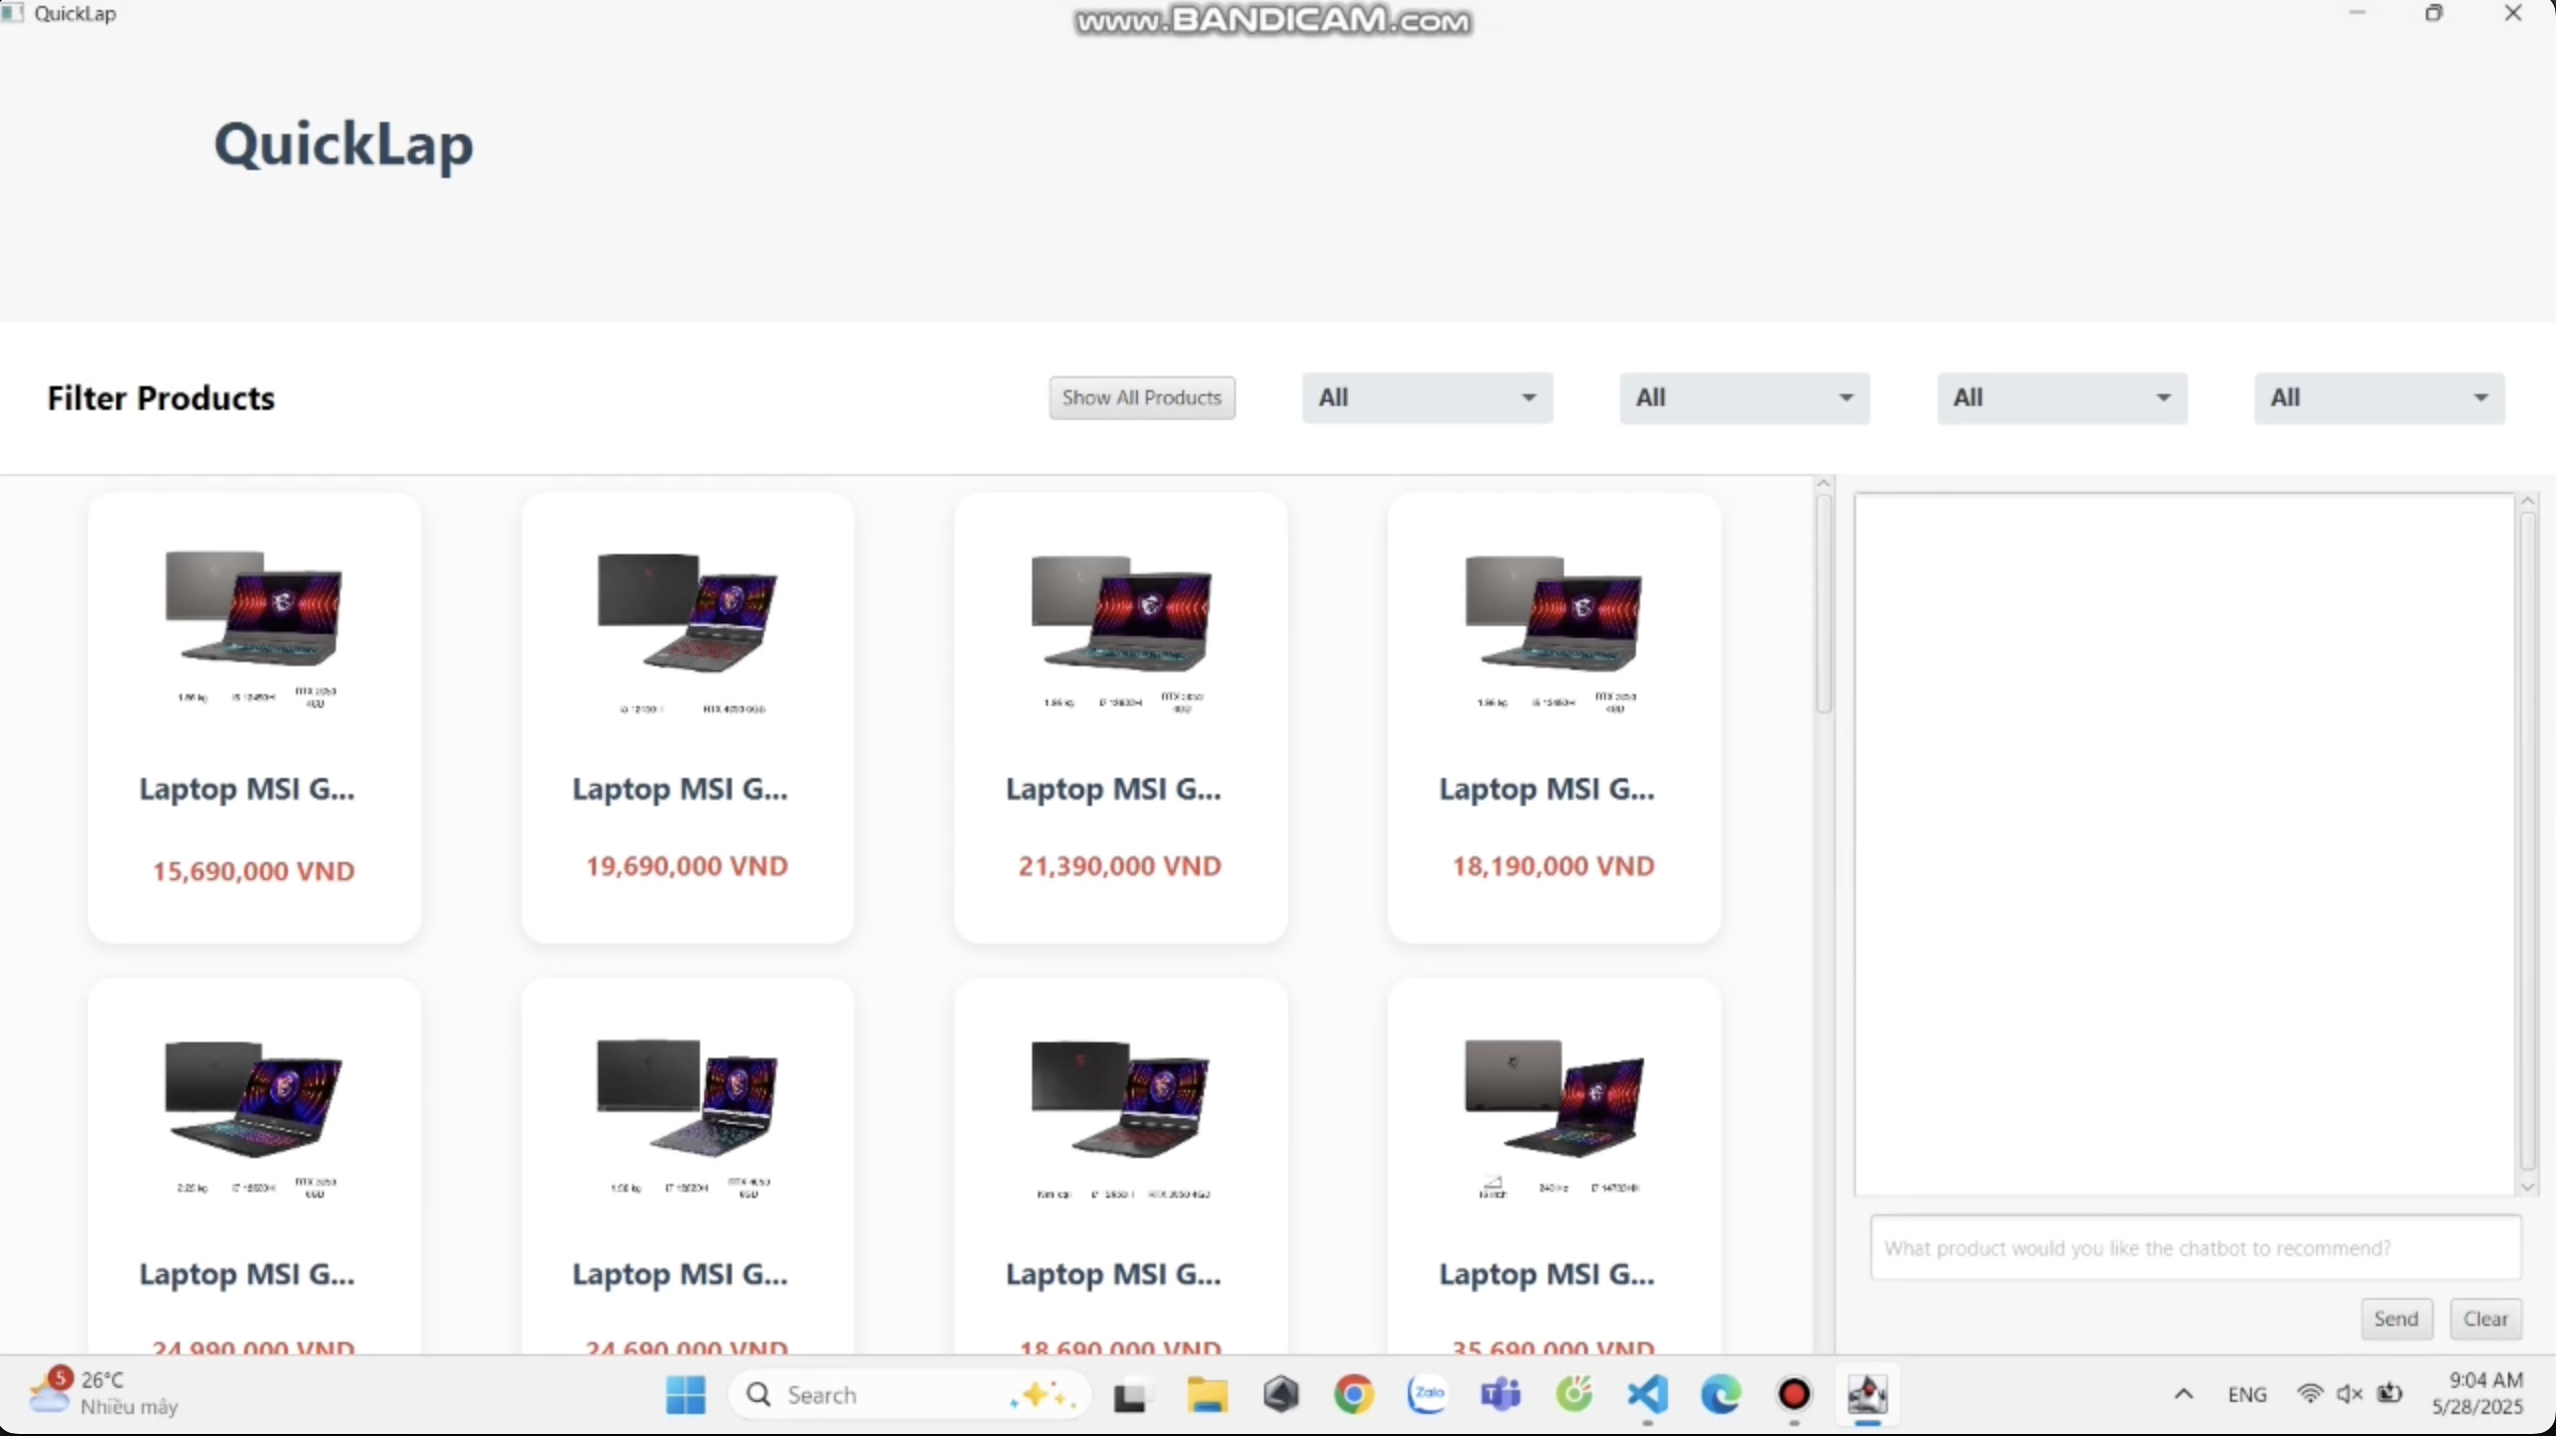
\includegraphics[width=\textwidth, keepaspectratio, center]{demo1.png} % Replace with actual screenshot
\\
\\
\\
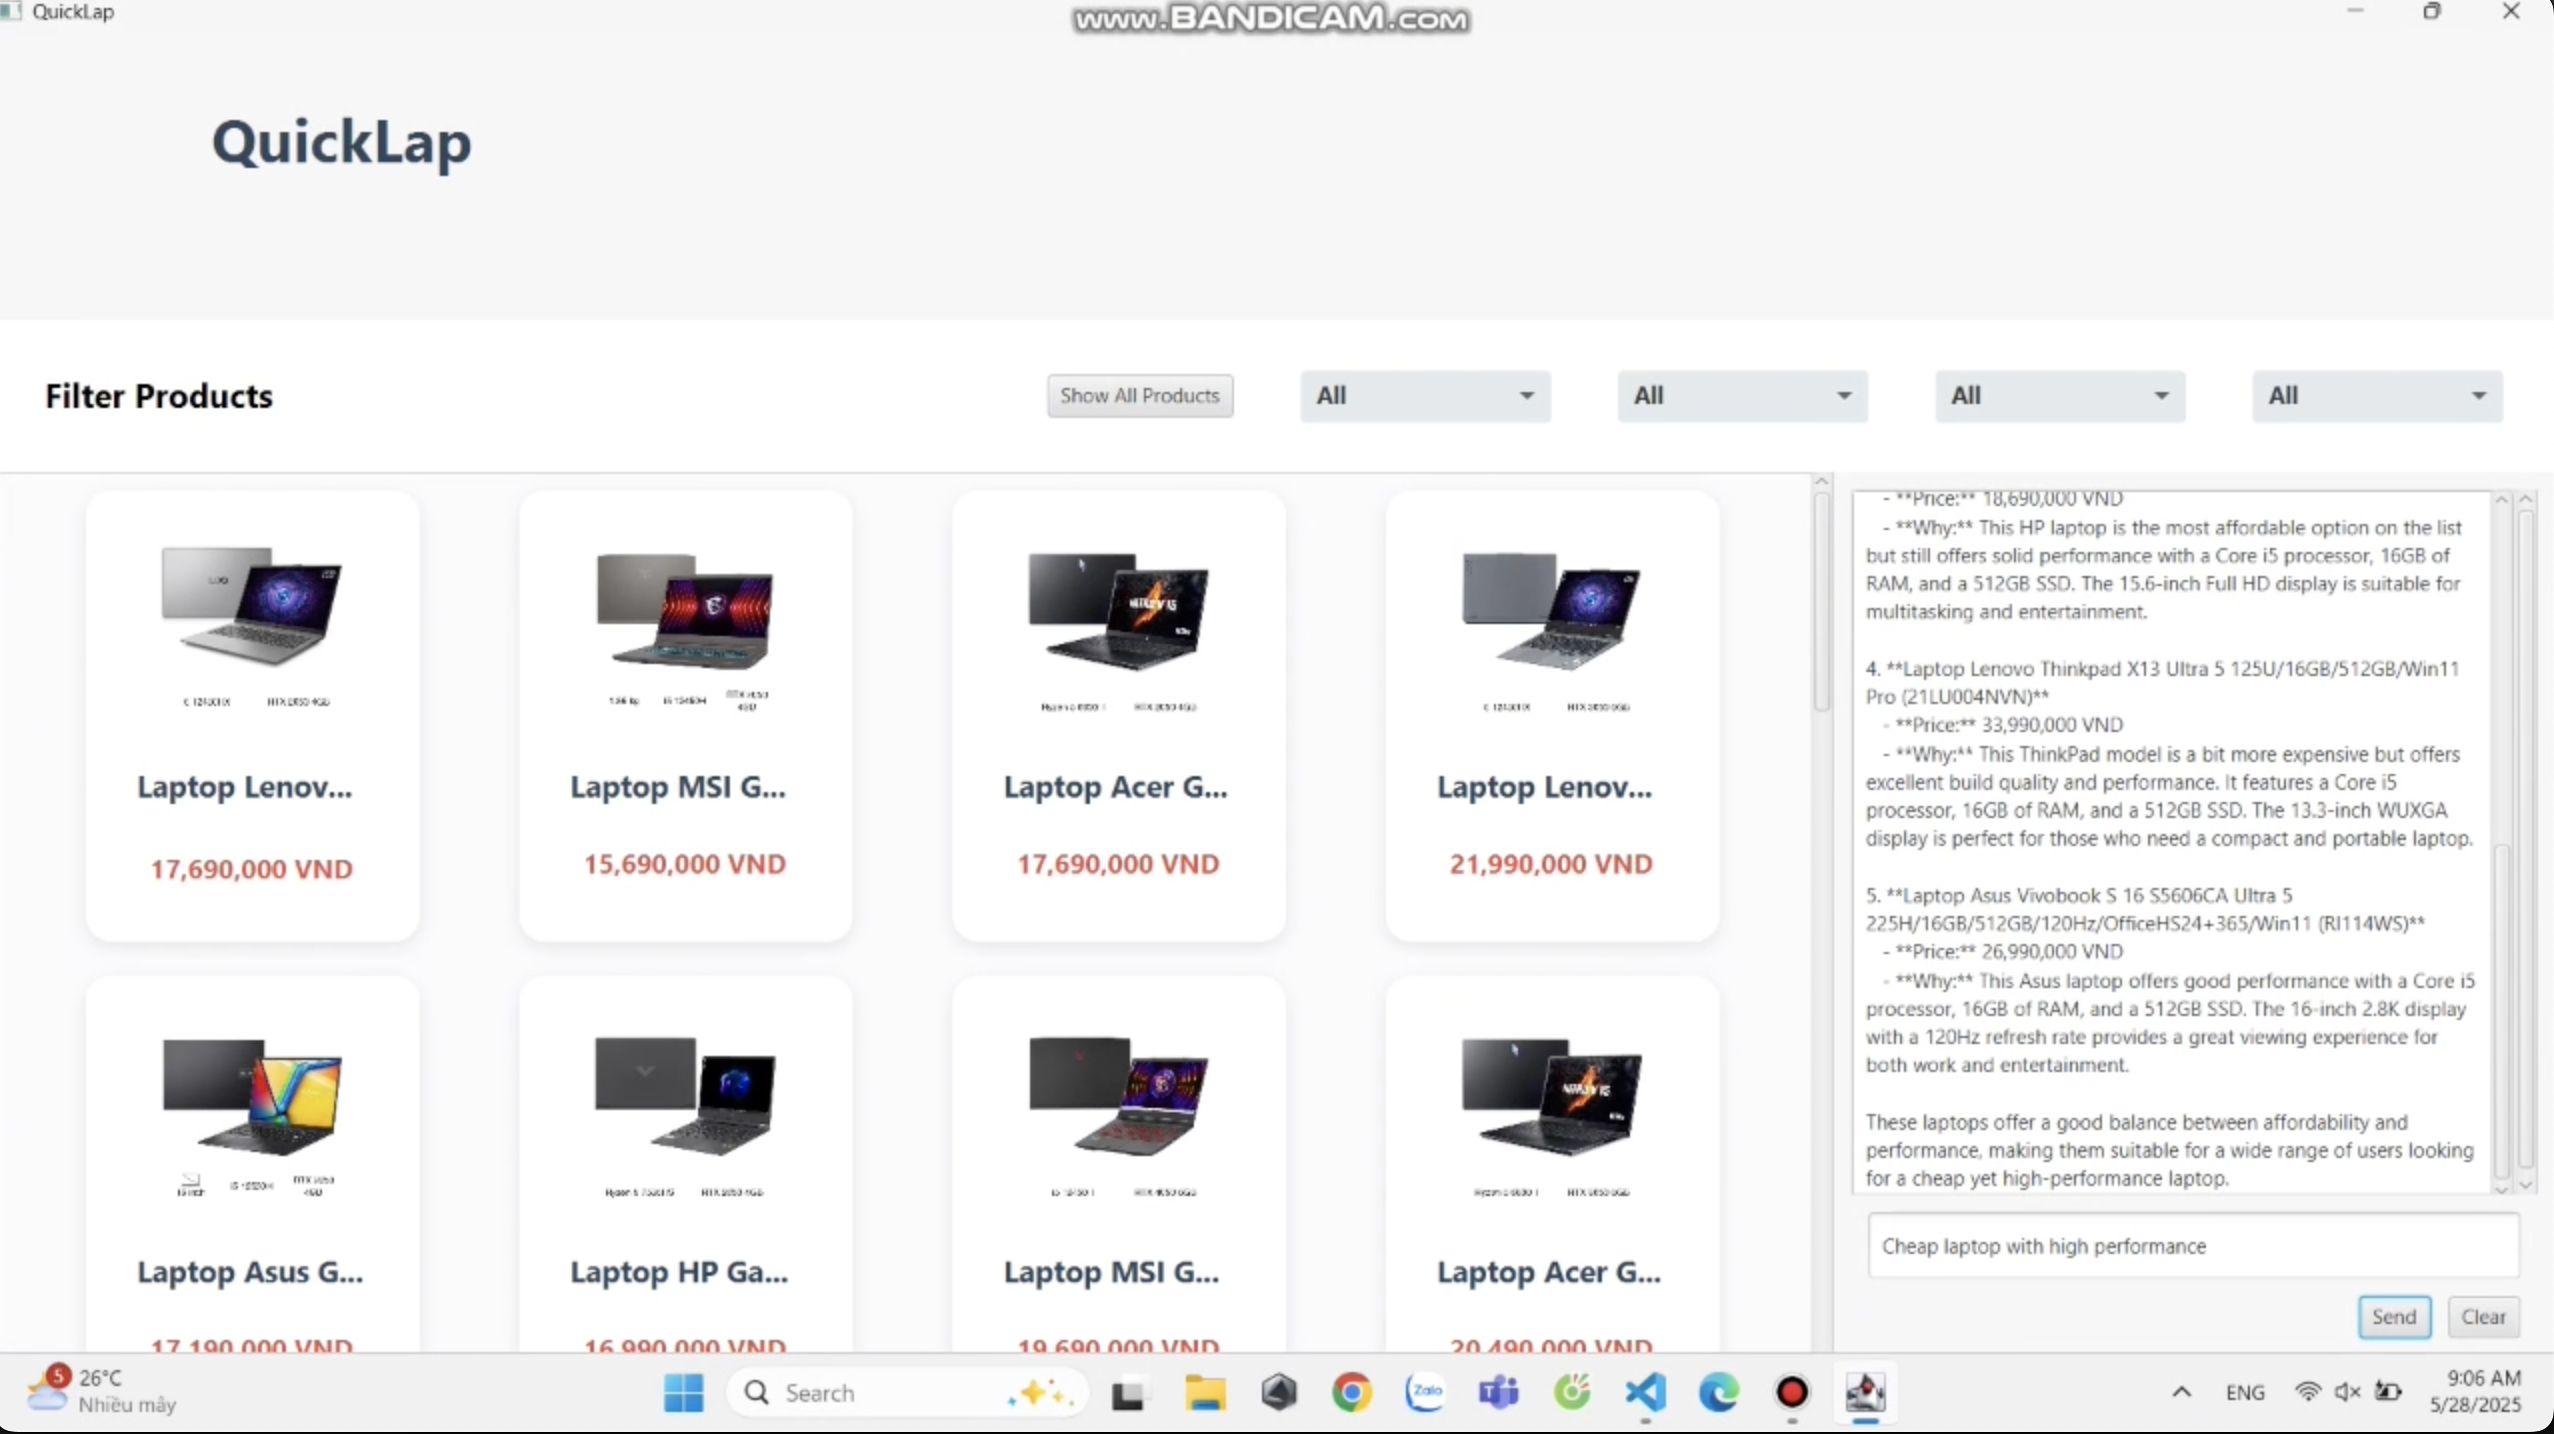
\includegraphics[width=\textwidth, keepaspectratio, center]{demo2.png} % Replace with actual screenshot

\newpage
\section{Conclusion}
\hspace{0.5cm}This project successfully developed a comprehensive Java-based desktop application designed to enhance the user's experience in discovering and learning about laptop products. By integrating a robust data collection pipeline, an intuitive JavaFX user interface, and advanced AI-driven features, the application provides a powerful tool for both casual browsing and specific product inquiry.

\subsection*{Achievements:}
\begin{itemize}
    \item \textbf{Automated Data Acquisition:} The successful implementation of a Selenium-based web scraper demonstrates an effective method for gathering up-to-date product information, which is then structured and persisted in a PostgreSQL database. This forms a reliable foundation for the application's data needs.
    \item \textbf{Intelligent Information Retrieval:} The integration of vector embeddings and cosine similarity for product search allows users to find relevant laptops based on semantic understanding, moving beyond simple keyword matching. This significantly improves the quality and relevance of search results.
    \item \textbf{AI-Powered Conversational Assistance:} The incorporation of the Mistral AI LLM via an API provides users with an interactive chatbot capable of answering product-related questions and offering recommendations, making the information discovery process more engaging and efficient.
    \item \textbf{Modular and Maintainable Architecture:} The project's adherence to design patterns such as DAO, Factory, and a clear separation of concerns (UI, business logic, data access) results in a well-structured, maintainable, and extensible codebase. The use of JavaFX for the UI ensures a modern and responsive user experience.
    \item \textbf{Effective Technology Integration:} The project successfully brought together diverse technologies, including Java, JavaFX, Selenium, PostgreSQL, and external AI APIs, showcasing the ability to build complex systems by leveraging appropriate tools for each component.
\end{itemize}

While the application achieves its primary objectives, potential avenues for future development include expanding the product categories beyond laptops, developing a web-based version for broader accessibility, implementing user accounts for personalized recommendations, and further refining the AI's conversational abilities and analytical depth. 
\vspace{0.3cm}\\
The reliance on external website structures for scraping and external APIs for AI functionalities also presents considerations for long-term maintenance and operational costs.
\vspace{0.3cm}\\
In conclusion, this project serves as a strong proof-of-concept for an intelligent product consultation system. It effectively demonstrates the power of combining automated data gathering, sophisticated search algorithms, and conversational AI to create a valuable tool for consumers. 
\vspace{0.3cm}\\
The established architecture and technological foundation provide a solid platform for future enhancements and the development of even more sophisticated product discovery and advisory services.


\end{document}